	%====================================================================================================
	% ?????
	%====================================================================================================
	% TCC
	%----------------------------------------------------------------------------------------------------
	% Autor				: Jasane Schio
	% Orientador		: Gedson Faria
	% Co-Orientador		: Angelo Darcy
	% Instituição 		: UFMS - Universidade Federal do Mato Grosso do Sul
	% Departamento		: CPCX - Sistema de Informação
	%----------------------------------------------------------------------------------------------------
	% Data de criação	: 01 de Outubro de 2015
	%====================================================================================================
	%descrever problemas e as solucoes encontradas
	\definecolor{dkgreen}{rgb}{0,0.6,0}
	\definecolor{gray}{rgb}{0.5,0.5,0.5}
	\definecolor{mauve}{rgb}{0.58,0,0.82}
	
	\lstset{frame=tb,
		language=C++,
		aboveskip=3mm,
		belowskip=3mm,
		showstringspaces=false,
		columns=flexible,
		basicstyle={\small\ttfamily},
		numbers=none,
		numberstyle=\tiny\color{gray},
		keywordstyle=\color{blue},
		commentstyle=\color{dkgreen},
		stringstyle=\color{mauve},
		breaklines=true,
		breakatwhitespace=true,
		tabsize=3
	}
	\chapter{Desenvolvimento} 
	
			Para o desenvolvimento foi escolhida a biblioteca OpenCV por ser OpenSource, multiplataforma, conter uma grande quantidade de métodos e algoritmos já implementados	e pelo seu rápido desempenho de máquina.
			A linguagem escolhida para o desenvolvimento foi o C++ pois é uma linguagem de programação compilada, o que torna sua execução mais rápida que as linguagem interpretadas, dando ao sistema grande desempenho, e por ser uma linguagem orientada objeto. 
			
			O sistema desenvolvido é separado em duas partes: Processamento e Interface Gráfica.
			A parte de Processamento é onde são feitas as partes de aquisição de imagem, processamento de imagem, conversão de imagem para modelo de cor HSV, seleção de pontos de cor e contagem de ocorrência de cor. Já a interface gráfica, é a onde ocorre a entrada do usuário para assim ser feita a calibração manual de mínimos e máximos de cada cor.
		
	
	Passos do projeto:
	\begin{description}
		\item[Aquisição de imagens em vídeo:] Nesse passo as imagem são adquiridas via câmera USB.
		
		\item[Identificação de Objetos:]
				 Durante o processo de aquisição de imagem são selecionados os objetos, quais serão usados como base para a detecção de máximos e mínimos de cores.
		\item [Cálculo de Mínimos e Máximos:]
		 Nessa etapa são levados em consideração os objetos teste. A imagem é percorrida pixel a pixel na localidade dos objetos-teste e assim são salvos seus valores e feito a contagem de ocorrências de cada cor.		
	\end{description}

\section{Tecnologias Usadas}
Para realização deste trabalho, irei utilizar a biblioteca de processamentos de imagens conhecida como OpenCV: Open Source Computer Vision Library. O trabalho será elaborado na linguagem C++, com uso do framework Qt para sua interface gráfica.
Os passos detalhados do projeto e seu desenvolvimento estará presente no Capítulo de Metodologia.
\begin{description}
	\item[OpenCV] Lançado em 1999 pela Intel\cite{Culjak:2012}, com objetivo de ser otimizada, portável e com um grande número de funções, o Open Source Computer Vision Library,OpenCV, se tornou se tornou uma ferramenta que possui mais de 2500 algoritmos e 40 mil pessoas em seu grupo de usuários\cite{Culjak:2012}. Já possui interface para as linguagens C++, C, Python e Java além de suporte para as principais plataformas com Windows, Linux, Mac OS, iOS e Android. A biblioteca lida tanto com imagens em tempo real, como vídeos e imagens estáticas.
	
	\item[Qt] Qt é um framework de desenvolvimento de aplicações multiplataforma. Entre suas funcionalidades está a possibilidade de criar interfaces gráficas diretamente em C ++ usando seu módulo Widgets.
	
	\item [C++] A linguagem de programação C++ foi projetado por Bjarne Stroustrup para fornecer eficiência e flexibilidade da linguagem C para programação de sistemas. A linguagem evoluiu a partir de uma versão anterior chamado C com Classes, o projeto C com Classes durou entre 1979 e 1983 e determinou os moldes para o C++. A linguagem foi oficialmente lancada em 1986.\cite{Stroustrup:1996} 
\end{description}

	\section{Projeto}
	\subsection{Organização do Projeto}
	 O projeto foi desenvolvido seguindo o paradigma de programação conhecido como  Orientação à Objetos, esse paradigma baseia-se na utilização de objetos individuais para criação de um sistema maior e complexo. A IDE usada para o desenvolvimento foi a QT Creator, esta separada o projeto em três pastas, Headers, Sources e Forms. Na pasta Headers estão os arquivos de cabeçalho(.h) onde estão as declarações dos métodos e variáveis usados nas classes  executáveis. Já na pasta Sources estão os arquivos fonte(.cpp), são nesses arquivos que os métodos declarados nos arquivos da pasta Header são implementados. Na pasta Forms está o arquivo de interface gráfica(.ui) que é usado no projeto para ser a ponte entre o usuario e as funções do sistema.
	 
	\begin{figure}[!h]
		\centering
		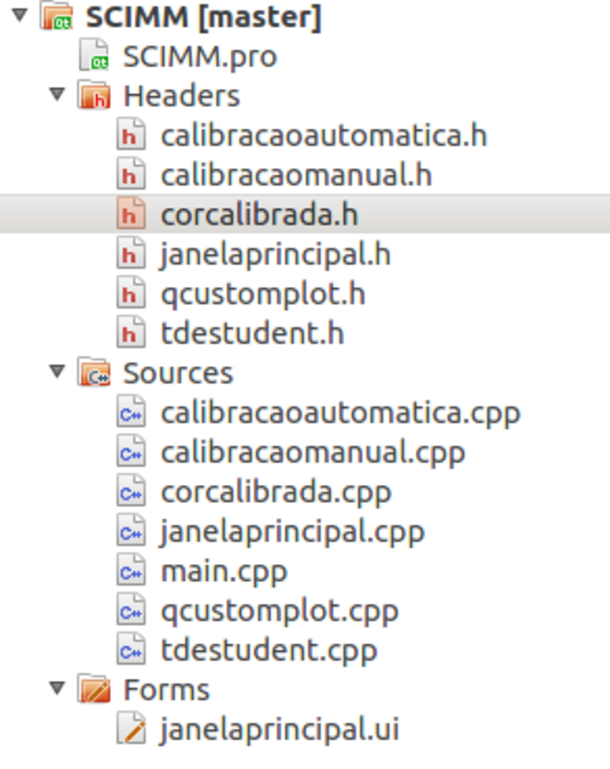
\includegraphics[width=0.2\textwidth]{organizacaoProjeto.pdf}
		\caption{Organização das pastas do projeto}
		\label{Organizacao do Projeto}
	\end{figure}
	Cada arquivo de cabeçalho possui um arquivo fonte correspondente, formando assim uma Classe, com exceção do arquivo fonte main, pois para este arquivo não há a necessidade.
	As classes desenvolvidas no projeto são:
 calibracao, manual, automatica, corcalibrada, janelaprincipal e tdestudent. Já a classe qcustomplot é um componente para auxilio em plotagem de gráficos e vizualização de dados\cite{QCustomPlot}.
Para melhor entendimento da interação entre as classes a figura 3.2 trás o diagrama de classes do projeto.
	 \begin{figure}[!h]
	 	\centering
	 	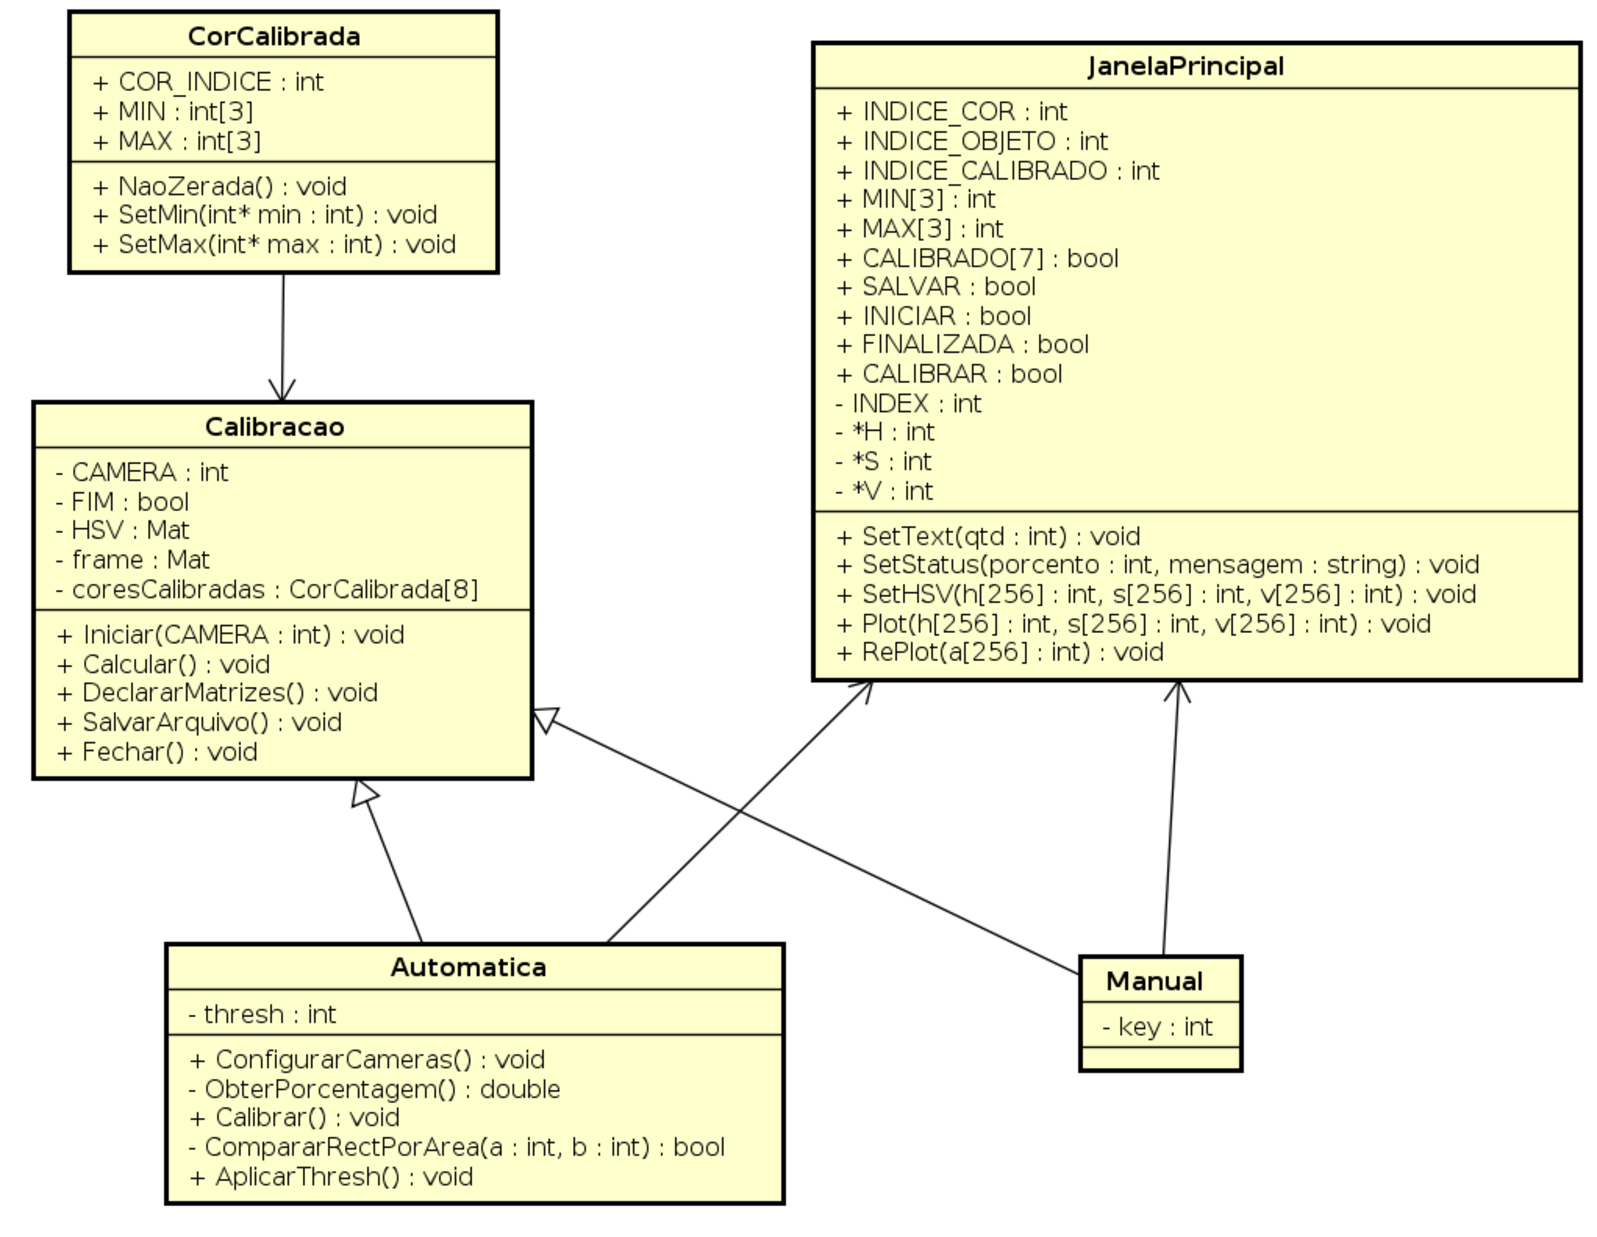
\includegraphics[width=0.8\textwidth]{diagramadeclasse.pdf}
	 	\caption{Diagrama de Classes do projeto}
	 	\label{DiagramaDeClasse}
	 \end{figure}\newpage


\subsection{Classes}
	\begin{description}

	\item [main] esta é a classe executavel do sistema, ela inicia o programa e em seguida chama a classe de interação grafica \textbf{janelaprincipal}  
	
	\item [janelaprincipal]	classe que faz a interação com o usuario e que de acorco com esta interação seleciona o tipo de calibração, e seus parametros, para então ser feita a analise dos pixeis	
		
	\item [calibracao] classe base que contem os metodos e variaveis que virão a ser usadas por ambas as classes \textbf{manual} e \textbf{automatica}
	
	\item [manual] classe que contem os metodos, cálculo e variaveis necessarias para a calibração manual
	
	\item [automatica] classe que contem os metodos, cálculo e variaveis necessarias para a calibração automatica
			
	\item [corcalibrada] classe que salva o indice da cor já calibrada e seu intervalo de valores
	
	\item [tdestudent] esta é a classe que faz o cálculo probabilistico conhecido com TdeStudent
	

	\end{description}

	

	\section{O Sistema}

		\begin{figure}[!h]
			\centering
			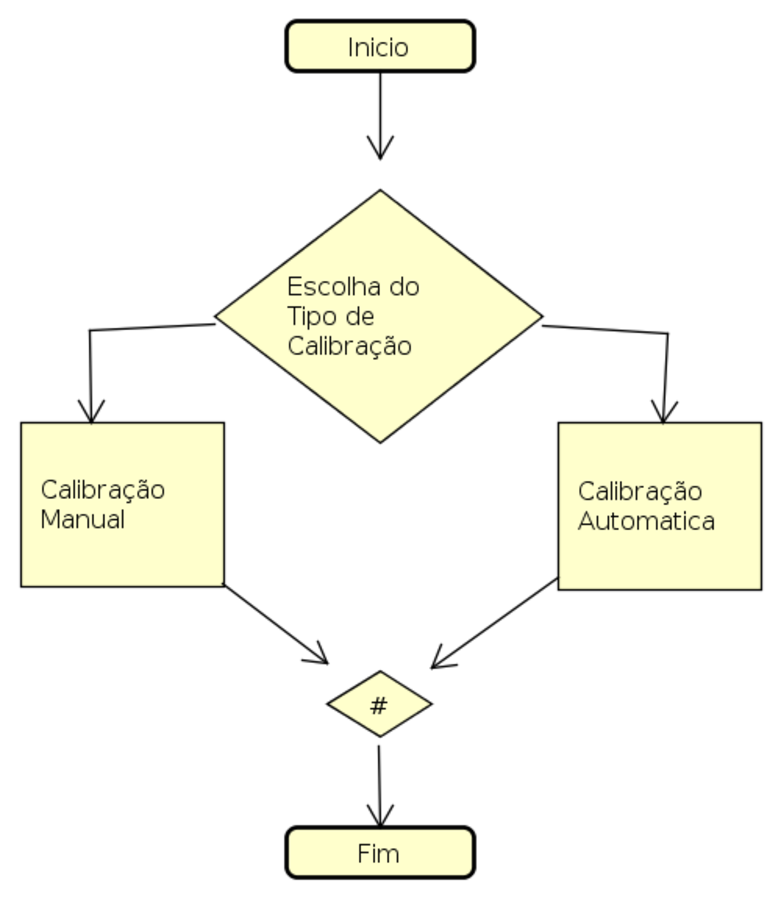
\includegraphics[width=0.45\textwidth]{fluxoprincipal.pdf}
			\caption{Diagrama de Fluxo}
			\label{FlowCHart}
		\end{figure}
		A Figura 3.3 mostra o diagrama de fluxo do sistema, este com duas possibilidades: Calibração Manual e Calibração Automatica. Ambas são independentes uma da outra.  
		
		 O sistema consiste na apresentação da \textbf{interface gráfica} ao usuario. A \textbf{interface grafica} que por sua vez oferece as duas possibilidades ao usuario, de acordo com o tipo de calibração escolhido o sistema inicia a rotina de calibração referente. Apos a execução de toda o sistema é finalizada.
			
	\subsection{Calibração Automatica}	
		\begin{figure}[!h]
					\centering
					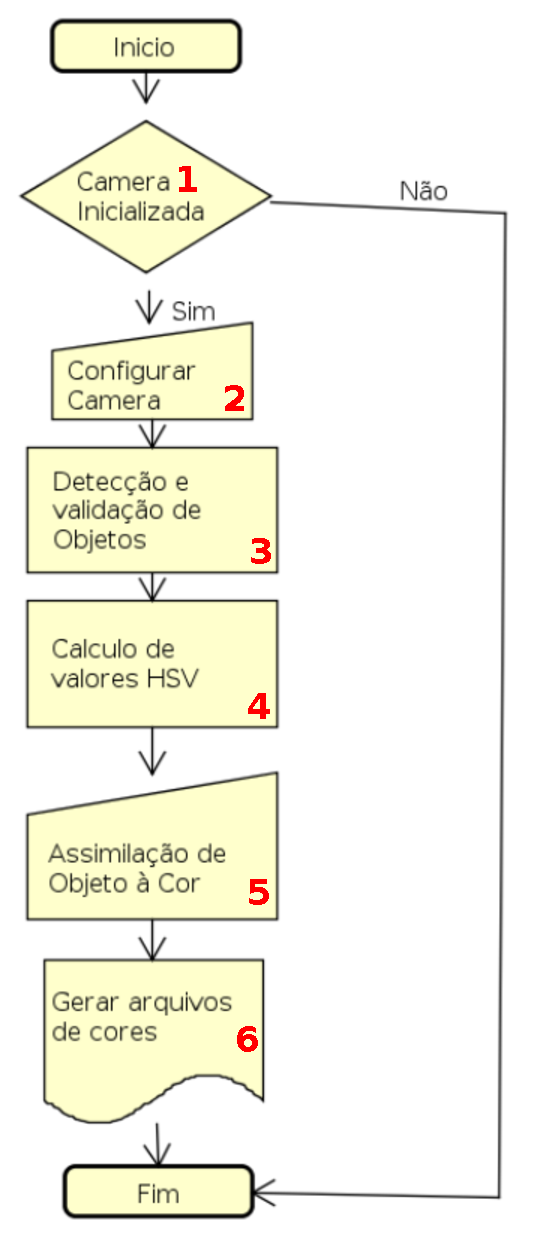
\includegraphics[width=0.45\textwidth]{fluxoautomatico.pdf}
					\caption{Diagrama de Fluxo Automatico}
					\label{DiagramaDeFluxoAutomatico}
				\end{figure} 
		Conformo mostrado na Figura \ref{DiagramaDeFluxoAutomatico} a rotina de calibração automatica possui cinco etapas. Este tipo de calibração  possui o mínimo possivel de interação com o usuario. O sistema faz automaticamente a detecção de objetos e utilizando a probabilidade matematica T de Student, considerando o tamanho de todos os objetos encontrados para encontrar os tamanhos minimo e maximo que os objetos desejados devem ter, nesse caso as etiquetas de cores dos robos, e só após determinar quais objetos possuem o tamanho desejado, analisar os valores e calcular as ocorrencias de cada um dos três valores do modelo HSV.
			
%	O fluxo inicia somente caso a camera esteja disponivel(1), apos a sua inicialização é feita a configuração da camera(2), enquadramento do tamanho correto e correção de brilho e luminosidade. Uma vez que a camera está configurada o sistema inicia a deteção de objetos e a validação dos objetos(3) que estão no tamanho correto. Apos deixar somente os objetos corretos no sistema, os pixeis de cada um são varridos e seu intervalo HSV encontrado(4). Os objetos e cores encontrados ficam disponiveis para o usuario apra esse fazer a assimilação entre os objetos e as cores corretas(5), após intervalos corretos já tiverem sido calibrados, um arquivo com os valores é gerado(6) e o usuario finaliza o sistema.
	
			
	Nas subsessões à seguir explicarei detalhadamente cada uma das etapas do processo de calibração automatica
	\subsubsection{1ª Etapa - Configuração de Camera}
Antes de ser feito a calibração propriamente dita são necessarias duas configurações: Ajuste de Constrate e Brilho e Recorte de Imagem.
A configuração de contraste e brilho utiliza o metodo \textit{convertTo} da biblioteca \textit{OpenCV} e é utilizada para o melhoramento da imagem antes da detecção dos objetos, a utilização completa fica da seguinte maneira:
\begin{center}
\centering \textit{ frameA.convertTo(frameA, -1, contrast\_value / 50.0, brightness\_value)}
\end{center}
Esta função recebe quatro parametros. O primeiro \textbf{frameA} informa aonde sera salvo o resultado da conversão. O segundo \textbf{-1} indica o tipo da matrix, ou numero de canais, da imagem a ser gerada, usa-se -1 quando se deseja que se use os valores semelhantes aos da imagem da imagem original\cite{OpenCV}, O terceiro \textbf{contrast\_value / 50.0} indica o valor de constraste, ou alpha, a ser usado para multiplicar os valores do pixel da imagem\cite{OpenCV} e por ultimo \textbf{brightness\_value} que é o valor do brilho, ou beta, a ser adicionado à imagem. \newline
Outra configuração feita é o Recorte de Imagem, onde utilizando a função setMouseCallback para possibilitar a interção do usuario na imagem por meio do mouse, sua utilização é dada da seguinte maneira:
\begin{center}
\centering \textit{ cv::setMouseCallback(src\_window,mouseHandler,0);}
\end{center}
Tem como primeiro parametro \textbf{src\_windows} que indica a janela na qual a função recebera a interação,  o segundo, \textbf{mouseHandler}, indica a função na qual esta implementada a interação e o ultimo parametro, \textbf{0}, indica parametros opcionais, neste caso não usaremos nenhum então foi usado o numero 0.
Dentro da função \textbf{mouseHandler} são identificados os pontos iniciai e final da seleção na tela e utilizada a função \textit{rectangle} para demarcar a seleção na tela. A utilização da função \textit{rectangle} completa fica da seguinte maneira:
\begin{center}
\centering \textit{ cv::rectangle(frameA, point1, point2, CV\_RGB(255, 0, 0), 2, 5, 0);}
\end{center}
A função rebece os parametros \textbf{frameA} indicando a imagem na qual será demarcada a area selecionada, depois o parametro \textbf{point1} que é o ponto incial de seleção na imagem, \textbf{point2} que é o ponto final da seleção. \textbf{CV\_RGB(255, 0, 0)} que indica a cor da demarcação, \textbf{2} indicando a expessura da demarcação, \textbf{5} que significa o tipo de linha a ser utilizado na demarcação e \textbf{0} que é o numero de bits fracinarios.
 Após confirmada a escolha do tamanho da tela 
este é então salvo na variavel nomeada \textit{tamanho}, está então sera usado durante todo o processo de calibração.
\newpage
\subsubsection{2ª Etapa - Detecção e validação de Objetos}
A detecção dos objetos a serem calibrados é dada pelo algoritmo de detecção de bordas de Canny. Como mais um recurso para eliminação de ruidos e melhoria da imagem antes de ser executado a detecção de objetos atravez da detecção de bordas é utilizado desfoque na imagem. O algoritmo de Canny já está implementado dentro da biblioteca OpenCV e com a seguite usagem:
\begin{center}
\centering \textit{  Canny(src\_gray, canny\_output, thresh, thresh * 3, 3);}
\end{center}
O algoritmo de Canny utiliza por padrão imagem em padrões de cinza, sendo assim \textbf{src\_gray} é a imagem orignal tranformada para escala de cinza, esta é a imagem na qual o algoritmo sera aplicado. \textbf{canny\_output} será a imagem de saida da função.
\textbf{thresh} e \textbf{thresh*3} são os limites mínimos e máximos para considerar uma borda. \textbf{3} é o valor de apertura ou kernel, o valor 3 é utilizado como padro.

Apos o uso do algoritmo de Canny para detecção de bordas é necessario então fazer uso da função \textit{findContours}, nativa no \textit{OpenCV} para detecção de contornos.
\begin{center}
\centering \textit{ findContours(canny\_output, contours, hierarchy, CV\_RETR\_EXTERNAL, CV\_CHAIN\_APPROX\_SIMPLE, Point(0, 0))}
\end{center}

O primeiro parametro, \textbf{canny\_output}, é a imagem que o algoritmo de Canny gerou com as bordas encontrada na imagem, e é a imagem que o método \textit{findContours} ira utilizar para detectar os contornos, \textbf{contours} é o parametro que indica onde serão salvos os contornos encontrados, cada contorno é armazenado como sendo um vetor de pontos \cite{OpenCV}. \textbf{hierarchy} é onde será salva um verot de informações sobre a topologia da imagem, e terá como total de elementos o mesmo numero que o total de contornos encontrado\cite{OpenCV}. O quarto parametro, \textbf{CV\_RETR\_EXTERNAL} indica o modo de obtenção de contornos, nesse caso \textit{CV\_RETR\_EXTERNAL} indica que o metodo só obtera os contornos exteriores\cite{OpenCV}. \textbf{CV\_CHAIN\_APPROX\_SIMPLE} indica o metodo que sera usado para aproximação de contornos, o metodo \textit{CV\_CHAIN\_APPROX\_SIMPLE} comprime segmentos horizontais, verticais, diagonais e deixa apenas os seus pontos finais\cite{OpenCV}. E o ultimo parametro, \textbf{Point(0, 0)}, indica o valor a ser usado para deslocar a imagem ao encontrar os objetos, neste caso esse valor é 0 para Y e 0 para X, pois não sera necessario. 

Uma vez obtidos os contornos é necessarios que se faça a eliminação de vertices dos polignos encontrados nos objetos deixando assim o objeto mais preciso. Isso é necessario para deixar a forma encontrada mais precisa dá forma original. Para este ajuste foi usado o metodo \textit{approxPolyDP}, ja implementado dentro da biblioteca OpenCV. Esse metodo teve que ser aplicado em cada um dos contornos encontrados, e foi utilizado da seguinte maneira:
\begin{center}
\centering \textit{    approxPolyDP(Mat(contours[i]), contours\_poly[i], 3, true)}
\end{center}
 Onde o metodo inicia recebendo como paralametro, \textbf{Mat(contours[i])} que é a criação de uma nova imagem, somente com aquele unico objeto, que esta sendo analisado. A seguir é informado no segundo parametro a variavel de destino \textbf{contours\_poly[i]}, onde sera salvo o objeto com a eliminação dos vertices. O terceiro parametro indica o valor do \textit{epilson}, usado o valor \textbf{3} que especifica a precisão da aproximação, a distância máxima entre a curva original e a sua aproximação\cite{OpenCV}. O ultimo parametro indica se a curva aparoximada sera fechada ou não, foi usado o valor \textbf{true} pois neste caso fechar um uma curva é necessario para que o objeto onde está a cor, seja idenficado e analisado na probabilidade.
 
 Por ultimo os objetos possuem sua borda ignorada, sendo assim calculado o tamanho interior dele, para que por ventura não hajam pixeis de cor preta ou derivadas a serem calculadas.
 
 A detecção de contorno detecta todos os contornos possiveis na imagem, isso inclue sombras, luzes entre outras coisas. Mas não são todos os objetos encontrados que deverão ser calculados, sendo assim foi usado o cálculo probabilistico T de Student.
 Foi implementado uma biblioteca para o uso da probabilidade voltada para objetos Rect, os objetos da biblioteca \textbf{OpenCV} obtidos na detecção. Essa biblioteca analisa a lista de objetos encontrados na detecção e faz o cálculo dos limites, tamanho mínimo e máximo, dos objetos. Apos a obtenção desse limite pela biblioteca são analisados todos os objetos encontrados na detecção e os cujo tamanho não esteja dentro deste limite são removidos da lista.
 
 \subsubsection{3ª Etapa - Calculo de valores HSV}
 Para que possam ser feitos os cálculo de valores HSV mínimo e máximos é necessario que se faça, primeiramente a conversão da imagem obtida pela camera, normalmente no espaço de cores RGB, para o espaço de cores HSV, pois a mesma lida melhor com deferenças de luminosidade. 
 A biblioteca \textbf{OpenCV} converte o espaço de cor usando a função \textit{cvtColor} que utiliza da imagem original, e de uma imagem vazia com memoria alocada para ser salva a imagem apos a conversão, além do parametro do tipo de conversão, Exemplo do uso do método:
\begin{center}
\centering \textit{cvtColor(frame, HSV, CV\_RGB2HSV);}
\end{center}

Apos a conversão é necessario, então, ser feita uma analise dos objetos encontrados. Para cada objeto serão somadas as ocorrencias de cada um dos valores, HSV, e salvos separadamente em um vetor para cada, H, S e V com 256 posiçoes, uma vez que se sabe que os valores de um pixel varial de 0 a 255. As ocorrençias são salvas se baseando no valor HSV do pixel. Para isso o pixel é separado em valores H, S e V este então tera seu valor correspondente a posição no vetor apropiado, por exemplo, se o valor de H em um determinado pixel for de 87, a posição de numero 87 no vetor ganhara uma ocorrencia a mais. No codigo, fica da seguinte maneira:
	        
	        \begin{algorithm}
	       		 \caption{Contagem dos Valores HSV}
		        \begin{algorithmic}
		     	
		     	\ForAll{objeto encontrado} 
		     		\ForAll{pixel do objeto} 
		   				 \State OcorrenciasDeH[pixel.h]++ 
		    			 \State	OcorrenciasDeS[pixel.s]++ 
		     	  		 \State	OcorrenciasDeV[pixel.v]++
		     	   \EndFor
		     	\EndFor
		     		
		        \end{algorithmic}
	        
	        \end{algorithm}
	        
        
Uma vez terminada a analise dos pixeis do objeto o sistema procupa o valor mínimo e máximo, ou seja a primeira e ultima ocorrencia. Esses valores são encontrados procurando o primeiro valor de pixel que não esta zerado e o ultimo valor que não esta zerado. Isto é feito para eliminar que durante a analise o numero de valores a serem comparados ao valor real do pixel, da imagem final, seja menor. Para exemplificar a Figura 3.6 tras o gráfico dos valores de H da calibração de um certo objeto antes de ser feia a eliminação dos valores. Se fosse analisado esses valores, não eliminando os valores zerados, o sistema buscaria no valor de H do pixel desde o valor 1 ao 126 sem a necessidade, pois se não houve ocorrencia desses valores no objeto de referencia, o que foi analisado, então esses valores não fazem parte da cor desejada.
% e tambem para remover ruidos de outros cores para que estas não interfiram na pureza da busca da dada cor.

\begin{figure}[!h]
	\centering
	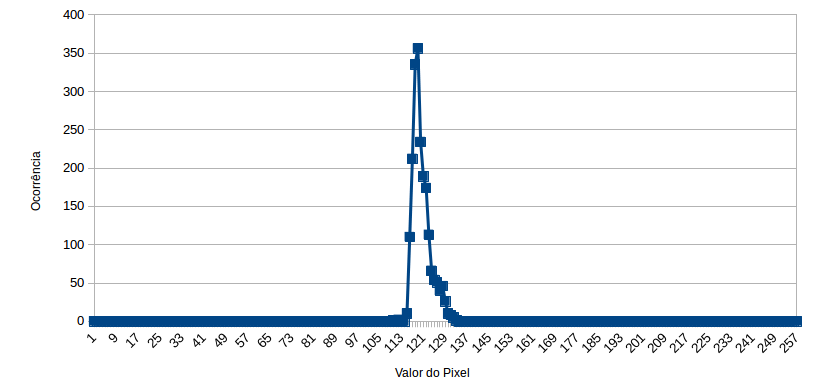
\includegraphics[width=0.5\textwidth]{graficototal.png}
	\caption{Grafico Exemplificando a Ocorrencia dos valores de H.}
	\label{Grafico Exemplo}
\end{figure}

 Apos ser feita a eliminação, Figura 3.7, de valos sabemos que somente a partir do pixel 110 houve ocorrencia, assim quando for necessario analisar pixel a pixel, os valores abaixo de 110 serão ignorados, ou seja não fazem parte da cor desejada.
 \begin{figure}[!h]
 	\centering
 	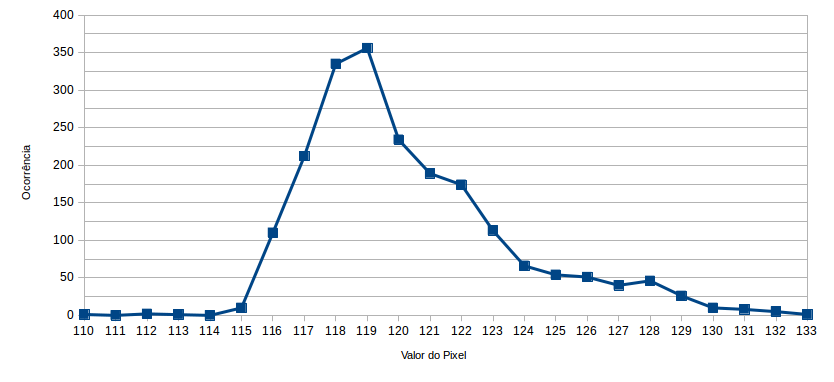
\includegraphics[width=0.5\textwidth]{graficominmax.png}
 	\caption{Grafico Exemplificando a Ocorrencia dos valores de H após eliminação.}
 	\label{Grafico Exemplo}
 \end{figure}

Após serem encontrados os valores mínimo e máximos para H, S e V de cada objeto detectado, estes valores são salvos em uma lista de objetos do tipo CorCalibrada. Neste objeto são salvos os respectivos valores.

 \subsubsection{4ª Etapa - Assimilação de Objeto à Cor}
 Uma vez que os objetos já foram identificados, suas cores analisadas e gerada sua lista. O sistema, utilizando do recurso de interface gráfica disponivel pela biblioteca Qt, informa ao usuario uma lista com os intervalos de cores encontrados, e outra lista com as possiveis cores a serem assimiladas para eles. Assim o usuario pode analisar um por um dos objetos e escolher qual se assemelha a qual cor. Assim que assimilada a cor ao objeto este é salvo e seu objeto CorCalibrada na lista de objetos salva o valor da cor em seu atributo COR\_INDICE.
 
  \subsubsection{5ª Etapa - Gerar Arquivo de Cores}
  Assim que todas as cores já estiverem sido assimiladas e a calibração finalizada, gera-se um arquivo chamado \textbf{cores.arff} contendo o indice de cada cor calibraa e seus valores máximos e mínimos.
  
  		
  	\subsection{Calibração Manual}
  	
  	  		\begin{figure}[!h]
  	  				\centering
  	  				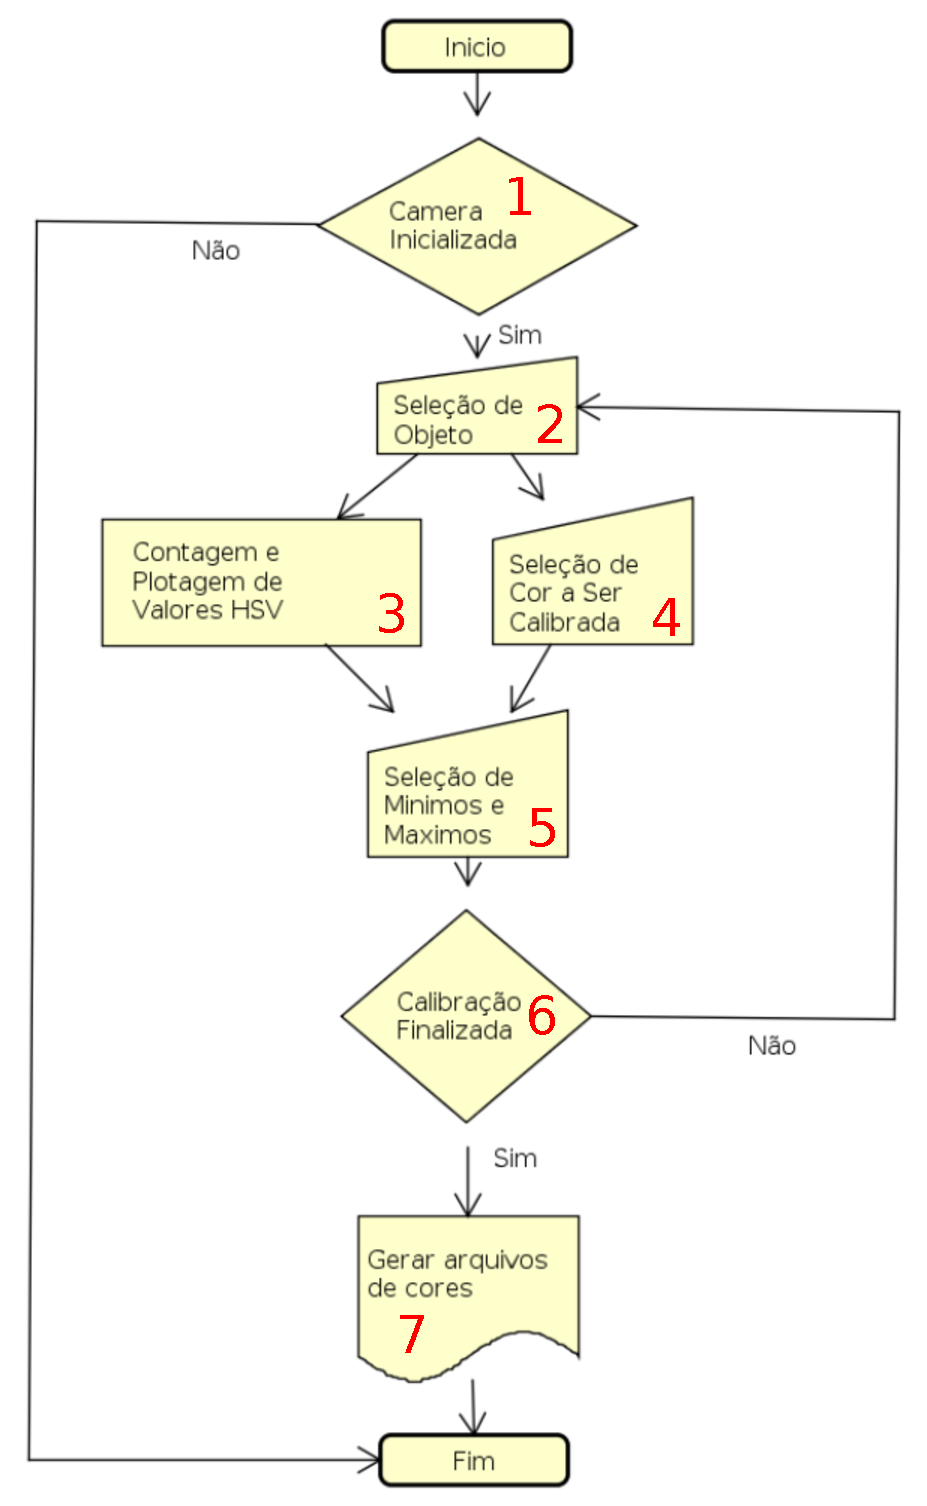
\includegraphics[width=0.45\textwidth]{fluxomanual.pdf}
  	  				\caption{Diagrama de Fluxo Manual}
  	  				\label{DiagramaDeFluxoManual}
  	  			\end{figure}
  	  		
  	  			
   A Figura \ref{DiagramaDeFluxoManual} mostra o fluxo de calibração manual, o sistema possui cinco etapas que permanecem em repetição até que todos os objetos sejam calibrados. Como o próprio nome já indica, o metodo de calibração é manual, sendo assim é necessario que o usuario selecione o objeto que o mesmo quer calibrar.
%   Após a camera ser inicializada(1) o sistema espera pela seleção do objeto(2) o qual tera seus pixeis calculados para gerar os valores HSV. Com o objeto selecionado o usuario escolhe então a cor(4), na opção de escolha de cor, e calibrar. A area selecionada é então analisada e os valores de cada pixel calculados analisando seu HSV(3).
%   	O usuario então seleciona os valores que considera satisfatorios(5). Enquanto houverem objetos a serem calibrados(6) o sistema repete esta mesma rotina, quando todos os objetos já tiverem sido calibrados, um arquivo com os valores é gerado(7) e o usuario finaliza o sistema.
	
  	\subsubsection{1ª Etapa - Seleção de Objeto}	
  	O primeiro passo para ser feita a calibração manual é a seleção de Objeto. Com o auxilio da função setMouseCallback, disponivel na biblioteca \textbf{OpenCV} e já explanada na sessão 3.2.1, é possivel obter os pontos de uma seleção feita na imagem, seu uso é necessario, já que obtenção de um ou mais objetos com a \textbf{mesma cor} a serem analisados é feita somente com a interação do usuario. Neste seleção existe a possibilidade de escolher somente um objeto ou mais de um objeto da mesma cor em diferentes pontos do campo, a seleção é feita somente um objeto por vez e cada objeto é analisado e seu valor e ocorrencia calculado utilizando o mesmo metodo encontrado na sessão 3.2.1 subsessão \textbf{Calculo de valores HSV}, estes valores são armazenados em memoria de execução e somente mostrados ao usuario quando requisitados. 
  	
  	\subsubsection{2ª Etapa - Plotagem de Valores HSV}	
  	Uma vez que o usuario já selecionou todos os objetos e os mesmos já foram analisados, o processo de calibração encaminha à interface grafica os valores encontrados e está plota três gráficos, um para cada um dos valores HSV.
  	Com a ajuda do componente auxiliar qcustomplot os gráficos são mostrados no sistema informando para o usuario quais foram os valores obtidos na seleção.
  	
  	\subsubsection{3ª Etapa - Seleção de Cor a ser Calibrada}
  	A seleção da cor na lista de cores possiveis para ser assimilado, pode ser considerada uma ação concomitante à ação de plotagem de graficos sendo que uma não depende dá outra, já que no momento da seleção do objeto o usuario já tinha em mente qual era sua cor, e a plotagem do gráfico não interfere nessa escolha, já a plotagem do gráfico é uma ação somente visual e não tem influencia da cor escolhida.
  	
  	\subsubsection{4ª Etapa - Seleção de Minimos e Maximos}
  	 Assim que os graficos são plotados, se torna então possivel, utilizando o recurso Slider, de fazer a seleção dos valores, tanto mínimo, quanto máximo. Ao ser modificado, cada um dos valores, o gráfico se ajusta para melhor detalhar ao usuario a ocorrencia dos pixeis. Ao contrario do sistema automatico, no sistema manual o objeto CorCalibrada só é criado após a seleção da cor e dos intervalos pelo usuario. Quando este salva a cor na interface gráfica, a mesma cor é encaminhada para o sistema manual e assim salva na lista.
  	 
  	 
\subsubsection{5ª Etapa - Gerar Arquivo de Cores}
Do mesmo modo que ocorre na calibração automatica, uma vez que todas as cores já estiverem sido assimiladas pelo usuario, este então finaliza a calibração e um arquivo com os valores calibrados é salvo localmente.
  	   	
  		
  	